\documentclass[12pt, a4paper]{article}
\usepackage[UTF8]{ctex}
\usepackage{amsmath}
\usepackage{amssymb}
\usepackage{amsthm}
\usepackage{geometry}
\usepackage{enumitem}
\usepackage{indentfirst}
\usepackage{caption}
\usepackage{fancyhdr}
\usepackage{booktabs}
\usepackage{titlesec}
\usepackage{draftwatermark}%水印
\usepackage{graphicx} % 导入图像的宏包、单图
% 页面布局设置
\geometry{top=2.54cm, bottom=2.54cm, left=3.18cm, right=3.18cm}

\SetWatermarkText{B站：布加拉提}
\SetWatermarkScale{0.4}

% 行距设置
\linespread{1.5}

% 段落设置
\setlength{\parindent}{2em}
\setlength{\parskip}{0.5em}

% 节标题格式设置
\titleformat{\section}{\normalfont\Large\bfseries}{第\chinese{section}章、}{1em}{}
\titlespacing{\section}{0pt}{2.5ex plus 1ex minus .2ex}{1.3ex plus .2ex}

% 定理环境设置
\newtheoremstyle{solution}
{}
{}
{}
{}
{\bfseries}
{、}
{1em}
{}
\theoremstyle{solution}
\newtheorem{sol}{解}

% 页眉页脚设置
\pagestyle{fancy}
\fancyhf{}
\fancyhead[C]{b站布加拉提整理（回忆版）b站甘茶w独家讲解}
\fancyfoot[C]{\thepage}

\rfoot{整理人：八方\\资源提供：考研乔瑟夫}
\lhead{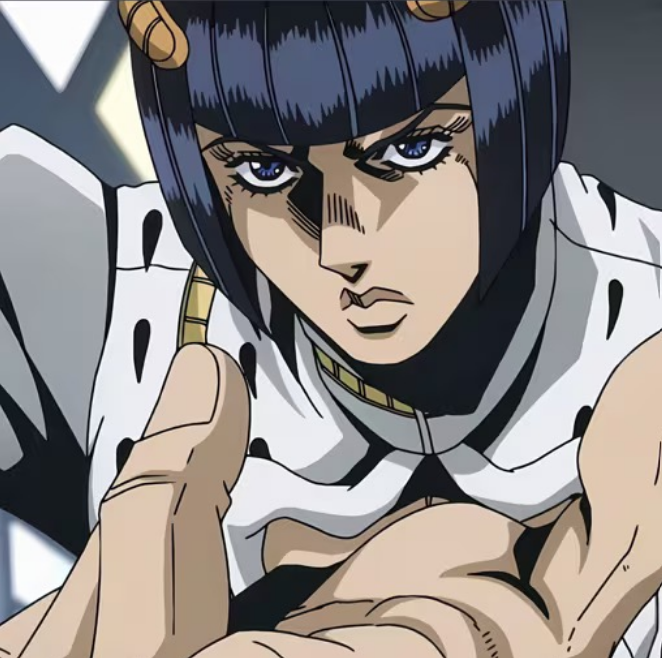
\includegraphics[width=0.06\linewidth]{p1.png}}
\rhead{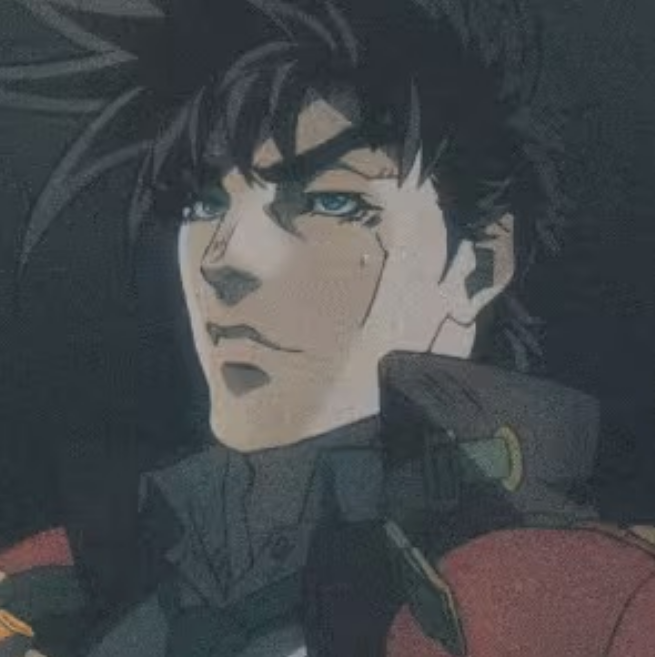
\includegraphics[width=0.06\linewidth]{p2.png}}
\renewcommand{\headrulewidth}{0.4pt}
\renewcommand{\footrulewidth}{0.4pt}

\begin{document}

\begin{center}
\Large\textbf{2020哈工大硕士考试试题：805物理光学}
\end{center}





\section*{一、填空题（20分）}
\begin{enumerate}
    \item 菲涅尔公式描述入射光和反射光，透射光之间\_\_\_\_\_和\_\_\_\_\_关系。
    \item 要使一束线偏振光通过偏振片之后振动方向转过90度，至少让这束光通过一块理想偏振片，在此情况下，最大透射光强与原来光强的比值是\_\_\_\_\_，若用一个元件来实现应该采用\_\_\_\_\_，其光轴与线偏振光成\_\_\_\_\_角度。
    \item 波动过程的基本特征可用\_\_\_\_\_，\_\_\_\_\_，\_\_\_\_\_三种现象表征。
    \item 产生干涉的条件是光波的\_\_\_\_\_。
    \item 产生全反射的条件是\_\_\_\_\_，当线偏振光以大于临界角入射时，反射光为\_\_\_\_\_偏振态。
    \item 若使观察衍射光谱的最大衍射角固定不变，将光栅的狭缝隔缝遮盖，光栅的分辨本领\_\_\_\_\_，自由光谱范围\_\_\_\_\_变化。
    \item 干涉发生的条件\_\_\_\_\_，\_\_\_\_\_，\_\_\_\_\_，\_\_\_\_\_。
    \item （大致）$x>y>z$是\_\_\_\_\_晶体。
\end{enumerate}
\section*{二、名词解释}
\begin{enumerate}
    \item 艾里斑
    \item 布儒斯特角
    \item 色散
    \item 双折射
    \item 倏逝波
\end{enumerate}
\section*{三、选择题}
\begin{enumerate}
    \item （重复）单轴晶体$e$光的折射率与$n_o,n_e$有关，除此之外还与其他相关的是\_\_\_\_\_。\\
    A.$e$光波法线与界面法线夹角\quad B.$e$光波法线与光轴夹角 \quad C.$e$光与界面法线夹角 \quad D.$e$光线与光轴夹角
    \item （重复）一束光是自然光和线偏振光的混合光，让它垂直通过一偏振片，若以此入射光束为轴旋转偏振光，测得透射光强度最大值是最小值5倍，那么入射光束中自然光和线偏振光的光强比值是\_\_\_\_\_.\\(A)1/2\qquad（B）1/5\qquad（C）1/4\qquad（D）2/3
    \item 当一束自然光以布儒斯特角入射到两种介质分界面上时，就偏振状态来说，反射光为\_\_\_\_\_，其振动方向\_\_\_\_\_入射面，透射光为\_\_\_\_\_。（以选择形式考察）
    \item 哪个物理量对双缝干涉的条纹间距没有影响？
    A.光波波长\quad B.缝距\quad C.双缝与光屏的距离\quad D.小孔的材料\quad
    \item 单轴晶体中o光e光的波阵面分别是\_\_\_\_\_。
    A.球面\quad B.旋转球面\quad C.旋转椭球面
\end{enumerate}
\section*{四、简答与计算题}
\begin{enumerate}
    \item （重复）给定光滑的玻璃表面和金属表面，问：自然光分别在两表面上反射，是否可以获得偏振光，条件是什么？偏振光分别在两表面上，反射光的偏振性质如何？为什么？
    \item （重复）什么是旋光效应？法拉第磁光效应和自然旋光现象有何不同，如何利用磁致旋光效应制作单通光闸？
    \item （重复） 以纳光观察迈克尔逊干涉条纹，先看到干涉场中12个亮环，且中心是亮点，然后移动一侧反射镜，看到中心消失了10个亮环，此时干涉场中还存在5个亮环。求：
    \begin{enumerate}
        \item 镜面移动的距离
        \item 开始时中心亮斑的级次$k_0$,相对应的等效空气薄膜厚$h_0$
    \end{enumerate}
    \item （重复）一个线偏振光在玻璃中传播时的表达式为：$E_z=0,E_y=0,E_x=(20V/m)(\pi\times10^{14}\times s^{-1}(t-\frac{x}{c})+\frac{\pi}{3})$,求该光的频率，波长，振幅，周期，初相位是多少？
    \item 什么是1/4波片？它有什么作用？用该器件是否能区分椭圆偏振光和部分偏振光？怎样区分？
    \item 一束偏振光$\lambda=589.6nm$垂直通过一块厚度为$1.618\times10^{-2}mm$的石英晶片。晶片折射率为$n_0=1.5442,n_e=1.5533$，光轴沿x轴1方向后，若入射光线偏振光的振动方向与x轴成45度，试决定出射光的偏振态。
    \item 根据瑞利判据，望远镜的分辨率，照相机物镜的分辨率，显微镜的分辨率分别是什么。如何增大显微镜的分辨率？
    \item 光谱仪的分辨率和成像系统的分辨率有何区别？
    \item 一束直径$2mm$的氦氖激光$\lambda=632.8nm$自地面发向月球，已知月球到地面的距离$3.76\times10^{5}km$，计算月球上接收到的光斑大小（涉及放大直径变$2m$与817类似，参考书课后题）。
    \item （情报缺失）干涉中三个有关距离公式
\end{enumerate}
\section*{六、论述题（10分）}
\begin{enumerate}
    \item (情报缺失)系统成像质量差，给出干涉装置检测哪里出问题
\end{enumerate}
\end{document}